\documentclass[../main.tex]{subfiles}

\begin{document}
%%%%%%%%%%%%%%%%%%%%%%%%%%%%%%%%%%%%%%%%%%%%%%%%%%%%%%%%%%%%%%%%%%%%%%%%%%%%%%%%%%%%%%%%
%                                                                                      %
% Integralrechnung II -- unbestimmtes Integral und Hauptsatz der Infinitesimalrechnung %
%                                                                                      %
%%%%%%%%%%%%%%%%%%%%%%%%%%%%%%%%%%%%%%%%%%%%%%%%%%%%%%%%%%%%%%%%%%%%%%%%%%%%%%%%%%%%%%%%

\chapter{SW09 Integralrechnung II -- unbestimmtes Integral und Hauptsatz der Infinitesimalrechnung}
\section{Unbestimmtes Integral und Flächenfunktion}
$I(x) = \int\limits_a^x f(t)dt$ \\
a ist ein bestimmter Wert, x ist unbestimmt. Darum unbestimmtes Integral.

\subsection{Theorem - unbestimmte Integrale}
\begin{itemize}
    \item Das unbestimmte Integral $I(x) = \int\limits_a^x f(t)dt$ stellt den Flächeninhalt zwischen
    $y=f(t)$ über dem Intervall $[a,x]$ in Abhängigkeit von der oberen Grenze $x$ dar.
    \item Zu jeder Funktion $f(t)$ gibt es $\infty$-viele unbestimmte Integrale, die sich nur
    durch ihre untere Grenze (a) unterscheiden.
    \item Die Differenz zweier unbestimmter Integrale $I_1(x)$ und $I_2(x)$ ist eine Konstante.
\end{itemize}
Die geom. Deutung als Fläche ist nur für $f(t)\geq 0$ und $x \geq a$ möglich. Man muss klar zwischen dem 
bestimmten Integral (das ist eine reelle Zahl) und dem unbestimmten Integral (das ist eine Funktion
der oberen Grenze) unterscheiden!

\subsection{Beispiel}
Zwei unbestimmte Integrale der Normalparabel $f(t)=t^2$ \\
$I_1(x)=\int\limits_0^x t^2dt$ und $I_2(x)=\int\limits_1^x t^2dt$ \\[7pt]
Deuten Sie den Unterschied $I_1(x) - I_2(x)$ geometrisch! \\
$A = I_1(x) - I_2(x) = \int\limits_0^1 t^2dt$

\section{Delta x ändern}
Wir lassen die unterschiedliche Bezeichnung zwischen der Integrationsvariabeln und der 
oberen Grenze fallen. Aus der Abb. liest man folgendes: \\
\begin{minipage}{0.5\textwidth}
    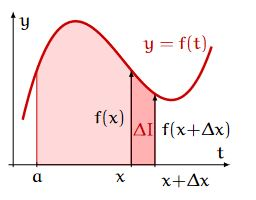
\includegraphics[width=50mm,scale=0.5]{deltax}
\end{minipage} \hfill
\begin{minipage}{0.45\textwidth}
    Einerseits hat man $\Delta I = I(x+\Delta x) - I(x)$ anderseits gilt die Approximation
    $\Delta I \approx f(x)\Delta x$. Also zusammengefasst: \\ [7pt]
    $f(x) \approx \frac{I(x+\Delta x) - I(x)}{\Delta x}$
\end{minipage}
Man kann zeigen, dass für stetige f gilt: \\ [7pt]
$f(x) = \lim\limits_{\Delta x \to 0} \frac{I(x+\Delta x) - I(x)}{\Delta x} = I'(x)$ \\ [7pt]
Wegen $I'(x) = f(x)$ ist also das unbestimmte Integral (oder die Flächenfunktion) $I(x)$ eine
Stammfunktion von $f(x)$.

\section{Fundamentalsatz der Differential- und Integralrechnung Theorem}
Jedes unbestimmte Integral $\int\limits_a^x f(t)dt$ der stetigen Funktion 
$f(x)$ ist eine Stammfunktion von $f(x)$: \\ [7pt]
$I(x) = \int\limits_a^x f(t)dt \Longrightarrow I'(x) = f(x)$. \\
Folgerungen aus dem Fundamentalsatz: \\
\begin{itemize}
    \item $I(x)$ ist wegen $I'(x) = f(x)$ eine stetig differenzierbare Funktion (falls f stetig).
    \item Jedes unbestimmte Integral hat die Form \\
    $I(x) = \int\limits_a^x f(t)dt = F(x) + C$ \\
    wobei $F(x)$ irgendeine (spezielle) Stammfunktion von $f(x)$ und $C_1$ eine 
    geeignete (reelle) Konstante bedeutet (die von a abhängt).
    \item Die Menge aller unbestimmter Integrale von $f(x)$ hat die Form \\
    $\int f(x)dx = F(x) + C$    $(F'(x)=f(x))$
    wobei $F(x)$ irgendeine (spezielle) Stammfunktion von $f(x)$ ist und $C \in \mathbb{R}$ alle
    reellen Werte durchläuft. Man nennt C Integrationskonstante.
    \item Für stetige Funktionen sind Stammfunktionen und unbestimmtes Integral das selbe.
\end{itemize}

\subsection{Beispiele}
$F_1(x) = \int (2x + 1)dx = x^2 + x + C$ \\ [7pt]
$F_2(x) = \int e^xdx = e^x + C$ \\ [7pt]
$F_3(x) = \int \frac{4}{1+x^2}dx = 4 \arctan(x) + C$ \\ [7pt]
$F_4(x) = \int \ln(x)dx = x \ln(x) - x + C$

\section{Berechnung bestimmter Integrale mit Stammfunktion}
Es gilt: \\
$I(x) = \int\limits_a^x f(t)dt = F(x) + C$ \\
$I(a) \int\limits_a^a f(x)dx = F(a) + C = 0 \longrightarrow C = -F(a)$ \\
somit gilt: \\
$I(x) = \int\limits_a^x f(t)dt = F(x) - F(a)$, und schliesslich $\int\limits_a^b f(t)dt = F(b) - F(a)$ \\
Das Integral hängt nicht von der Wahl der Stammfunktion $F(x)$ ab: man kann irgendeine (spezielle) Stammfunktion wählen!

\subsection{Beispiel}
Berechnen Sie die bestimmten Integrale $\int\limits_0^1 x^2dx$. \\
$\int\limits_0^1 x^2dx = \left[\frac{1}{3}x^3+C\right]_0^1 = (\frac{1}{3}1^3 + C) - (\frac{1}{3}0^3 +C) = \frac{1}{3} + C -0 -C = \frac{1}{3}$ \\
$\longrightarrow$ Hier beim bestimmten Integral zum Flächenberechnen kann man $+C$ weglassen (aber nur hier, da es sich immer rauskürzt)! \\
\\
Berechnen Sie die bestimmten Integrale $\int\limits_0^\pi \sin xdx$. \\
$\int\limits_0^\pi \sin xdx = \left[-\cos x \right]_0^\pi = -\left[\cos x \right]_0^\pi = -(\cos \pi - \cos 0) = -(-2) = 2$

\section{1. Substitutionsregel für unbestimmte Integrale - Theorem}
Es gilt: \\
$\int f(g(x))g'(x)dx = \left[ \int f(u)du\right]_{u=g(x)}$ \\
Vorgehen:
\begin{itemize}
    \item Substituiere formal $g(x) = u, g'(x)dx = du$
    \item Integriere unbestimmt nach u
    \item Ersetze u wieder durch $g(x)$
\end{itemize}

\subsection{Beispiele}
Berechne das unbestimmte Integral $I = \int(x^2+1)^{50}2xdx$ \\
$u = x^2+1$ \\
$\frac{du}{dx} = 2x$ \\
$du = 2xdx$ \\
$I = \int(x^2+1)^{50}2xdx = \int u^{50}du = \frac{1}{51}u^{51} + C = \frac{1}{51}(x^2+1)^{51} + C$
\\ [14pt]
Berechne das unbestimmte Integral $I = \int x \cos x^2 dx$ \\
$u = x^2$ \\
$\frac{du}{dx} = 2x$ \\
$du = 2xdx$ \\
$\int x \cos x^2 dx = \frac{1}{2}\int \cos x^2 2xdx = \frac{1}{2}\int \cos (u) du$
$ =  \frac{1}{2}\int \sin (u) + C = \frac{1}{2}\int \sin (x^2) + C$

\section{1. Substitutionsregel für bestimmte Integrale - Theorem}
Es gilt: \\
$\int\limits_a^b f(g(x)) g'(x)dx = \int\limits_{g(a)}^{g(b)} f(u)du$ \\
Vorgehen:
\begin{itemize}
    \item Substituiere formal $g(x) = u, g'(x)dx = du$
    \item Ersetze die x-Grenzen a,b durch die u-Grenzen $g(a),g(b)$
    \item Integriere
\end{itemize}

\subsection{Beispiele}
Berechne das bestimmte Integral $I = \int\limits_0^2 x(x^2+1)^3dx$ \\
$u = u(x)=  x^2 + 1$ \\
$\frac{du}{dx} = 2x$ \\
$du = 2xdx$ \\
$I = \int\limits_0^2 x(x^2+1)^3dx = \frac{1}{2} \int\limits_0^2 2x(x^2+1)^3dx$ \\
Intervallgrenzen: 2, 0. Neue Grenzen: $u(2)=5, u(0)=1$ \\
$\frac{1}{2} \int\limits_1^5 u^3du = \frac{1}{2} \left[ \frac{1}{4} u^4\right]_1^5$
$ = \frac{1}{8} \left[ u^4\right]_1^5 = \frac{1}{8}(625 - 1) = 78$
\\ [14pt]
Berechne das bestimmte Integral $I = \int\limits_0^{\frac{\pi}{3}}\frac{\cos x}{1 + 4\sin ^2 x}dx$ \\
$u = u(x)=  \sin x$ \\
$\frac{du}{dx} = \cos x$ \\
$du = \cos xdx$ \\
Intervallgrenzen: $\frac{\pi}{3}$, 0. Neue Grenzen: $u(\frac{\pi}{3})=\frac{\sqrt[]{3}}{2}, u(0)=0$ \\ [7pt]
$\int\limits_0^{\frac{\sqrt[]{3}}{2}} \frac{du}{a+4u^2}$
$\int\limits_0^{\frac{\sqrt[]{3}}{2}} \frac{du}{a+(2u)^2}$
$\frac{1}{2}\int\limits_0^{\frac{\sqrt[]{3}}{2}} \frac{2du}{a+(2u)^2}$ \\
$v = v(x)=  2u$ \\
$\frac{dv}{du} = 2$ \\
$dv = 2du$ \\
Intervallgrenzen: $\frac{\sqrt[]{3}}{2}$, $0$, neue Grenzen: $v(\frac{\sqrt[]{3}}{2}) = \sqrt{3}, v(0) = 0$ \\
$\frac{1}{2}\int\limits_0^{\sqrt[]{3}}\frac{dv}{1+v^2} = \frac{1}{2} \left[ \arctan (v)\right]_0^{\sqrt[]{3}}$
$ = \frac{1}{2}(\arctan \sqrt[]{3} - \arctan 0) = \frac{\pi}{6}$

\end{document}